\documentclass[12pt,letterpaper]{article}
\usepackage[utf8]{inputenc}
\usepackage[T1]{fontenc}
\usepackage{lmodern}
\usepackage[margin=1in]{geometry}
\usepackage{setspace}
\usepackage{parskip}
\usepackage{amsmath,amssymb}
\usepackage{booktabs}
\usepackage{graphicx}
\usepackage{xcolor}
\usepackage{enumitem}
\usepackage{hyperref}
\usepackage{float}

\hypersetup{colorlinks=true, linkcolor=blue!60!black, citecolor=blue!60!black, urlcolor=blue!60!black}
\onehalfspacing

\title{\textbf{Event Density as a Physical Ontology:\\[4pt] From Primitives to Dynamics to Empirical Predictions}}
\author{Allen Proxmire}
\date{March 2026}

\begin{document}
\maketitle
\thispagestyle{empty}

\begin{abstract}
\noindent
Event Density (ED) is a constitutive ontology built on the premise that physical structure arises from the local rate of becoming---the density of micro-events in spacetime. From four primitives (density, mobility, penalty, participation) and seven structural axioms, a unique canonical PDE is derived. This PDE decomposes into three constitutive channels---nonlinear diffusion, exponential relaxation, and telegraph oscillation---each corresponding exactly to a known physical law.

This paper synthesises two empirical programmes. In condensed matter, the ED mobility law $D(c) = D_0(1-c/c_{\max})^\beta$ fits three chemically distinct materials with $R^2 > 0.98$ and a mean exponent $\beta = 2.00 \pm 0.29$. The front-propagation exponent $\alpha_R = 1/(d\beta+2)$ is confirmed to 2.3\% in 1D.

At galactic scales, the ED PDE coupled to the Poisson equation produces density profiles with naturally widened cores matching observed Burkert core radii to within 10\%. The temporal-tension interpretation predicts indefinitely flat circular velocities consistent with Mistele et al.\ (2024) weak-lensing observations. The baryonic Tully--Fisher relation $V \propto M_b^{1/4}$ is derived as a temporal-tension amplitude scaling law, with the measured exponent $n = 0.246 \pm 0.025$ matching the prediction exactly. The ED acceleration scale $a_{\mathrm{ED}} = 2.1 \times 10^{-10}$~m/s$^2$ is within a factor of 1.8 of Milgrom's $a_0$.

Two tests uniquely distinguish ED from both MOND and $\Lambda$CDM: (1) activity-dependent weak-lensing velocities ($\Delta V \sim 30$--70~km/s), and (2) temporal-tension lensing lags in merging clusters (15--45~kpc behind the baryonic mass---opposite to the $\Lambda$CDM Bullet Cluster offset). Both tests are feasible with current surveys.
\end{abstract}

\newpage
\tableofcontents
\newpage

%========================================================================
\section{Introduction}
%========================================================================

\subsection{The Ontological Question}

Physics describes the world through equations. But equations require objects---fields, particles, metrics---and rules for how those objects interact. The choice of objects is an ontological choice: it determines what kind of structure the theory can produce.

General relativity begins with a metric tensor and a stress-energy source. Quantum mechanics begins with a Hilbert space and a Hamiltonian. The Standard Model begins with gauge fields and representations. Each ontology generates a specific class of phenomena. None generates them all from a single set of primitives.

Event Density asks: \emph{is there a simpler set of primitives---a constitutive architecture---from which the structural content of multiple physical theories can emerge?}

\subsection{Event Density as Ontology}

The ED ontology begins with a single scalar field: the local rate of becoming. At each point in space and time, things happen---interactions occur, fields fluctuate, particles scatter. The density of these micro-events is a real-valued scalar $\rho(x,t) \in [0, \rho_{\max}]$, bounded by a capacity limit.

From this primitive, three constitutive channels are derived:

\begin{enumerate}[leftmargin=2em]
\item \textbf{Mobility.} How density redistributes. Transport is density-dependent: it slows as $\rho$ approaches $\rho_{\max}$ and halts at the capacity bound, creating horizons and compact-support fronts.
\item \textbf{Penalty.} How density relaxes. A monostable restoring force drives $\rho$ toward a unique equilibrium $\rho^*$, producing exponential decay.
\item \textbf{Participation.} How the system oscillates. A global variable $v(t)$, driven by the domain-averaged density operator and feeding back uniformly, produces telegraph oscillations.
\end{enumerate}

These three channels, combined into a single PDE derived from seven axioms, generate a family of dynamics that includes exponential relaxation, self-similar spreading with compact support, free-boundary formation, oscillation-modulated diffusion, and effective pair interactions.

\subsection{Scope of This Paper}

This paper connects the ED ontology to empirical physics at two scales:

\begin{itemize}[leftmargin=2em]
\item \textbf{Condensed matter} (Sections~3--4): the ED mobility law is fitted to concentration-dependent diffusion data from three materials, confirming the functional form and exponent.
\item \textbf{Galaxy dynamics} (Sections~5--8): the ED PDE coupled to gravity reproduces dwarf galaxy halo profiles, and the temporal-tension channel predicts the baryonic Tully--Fisher relation and weak-lensing flatness to 1~Mpc.
\end{itemize}

Two tests that uniquely discriminate ED from MOND and $\Lambda$CDM are derived in Section~8.

%========================================================================
\section{The ED Dynamical Equation}
%========================================================================

\subsection{The Canonical PDE}

The canonical ED system on $\Omega \subset \mathbb{R}^d$ is:
\begin{align}
\partial_t\rho &= D\bigl[\nabla\cdot(M(\rho)\nabla\rho) - P(\rho)\bigr] + Hv, \label{eq:pde}\\
\dot{v} &= \frac{1}{\tau}(\bar{F} - \zeta v), \label{eq:vode}
\end{align}
with constitutive functions:
\begin{equation}
M(\rho) = M_0(\rho_{\max}-\rho)^\beta, \qquad P(\rho) = P_0(\rho - \rho^*). \label{eq:const}
\end{equation}

This PDE is the unique second-order, scalar, isotropic, dissipative system satisfying the seven architectural axioms:

\begin{itemize}[leftmargin=2em, itemsep=2pt]
\item \textbf{P1 (Locality).} The operator at each point depends only on $\rho$ and its derivatives at that point.
\item \textbf{P2 (Isotropy).} The operator is invariant under rotations and reflections.
\item \textbf{P3 (Gradient-driven flow).} The flux is $J = -M(\rho)\nabla\rho$ with state-dependent mobility $M(\rho) \geq 0$.
\item \textbf{P4 (Dissipative structure).} There exists a Lyapunov functional $E[\rho]$ with $dE/dt \leq 0$.
\item \textbf{P5 (Single scalar field).} The system evolves a single real-valued scalar $\rho(x,t)$.
\item \textbf{P6 (Minimal coupling).} The global mode $v(t)$ is driven by the domain-averaged operator and feeds back additively.
\item \textbf{P7 (Dimensional consistency).} The constitutive functions are independent of spatial dimension $d$.
\end{itemize}

The derivation proceeds by elimination: P1+P2 reduce the operator to functions of $(\rho, |\nabla\rho|^2, \nabla^2\rho)$; P3 determines the principal part as a divergence; P4 constrains the zeroth-order term to a monostable penalty; P5 excludes non-scalar fields; P6 determines the participation coupling; P7 ensures all constitutive functions are dimension-free.

\subsection{The Generalised Mobility}

For galaxy-scale applications, the mobility is extended to:
\begin{equation}
M(\rho) = \rho^\alpha(\rho_{\max}-\rho)^\beta, \label{eq:gen_mob}
\end{equation}
where $\alpha > 0$ suppresses transport at low density (steepening the outer halo) and $\beta > 0$ suppresses transport at high density (widening the core). The canonical ED ($\alpha = 0$) is recovered as a special case.

\subsection{Channel Correspondences}

\begin{table}[H]
\centering
\begin{tabular}{@{}llll@{}}
\toprule
Channel & Isolated equation & Physical law & Accuracy \\
\midrule
Penalty & $\dot{\delta} = -DP_0\delta$ & RC/Debye decay & \textbf{Exact} (0.00\%) \\
Mobility & $\partial_t\delta = D_{\mathrm{pme}}\nabla^2(\delta^m)$ & PME ($m=\beta+1$) & \textbf{Exact reduction} \\
Participation & $\ddot{\delta}+2\gamma\dot{\delta}+\omega_0^2\delta=0$ & RLC telegraph & \textbf{Exact} (0.00\%) \\
\bottomrule
\end{tabular}
\caption{Each ED channel corresponds exactly to a known physical law.}
\end{table}

These are mathematical identities, not analogies.

%========================================================================
\section{Mapping ED to Condensed Matter}
%========================================================================

\subsection{The Testable Prediction}

The ED mobility law predicts:
\begin{equation}
\frac{D(c)}{D_0} = \left(1-\frac{c}{c_{\max}}\right)^\beta. \label{eq:mob_law}
\end{equation}

\subsection{Three-Material Universality Test}

\begin{table}[H]
\centering
\begin{tabular}{@{}llccc@{}}
\toprule
Material & Mechanism & $\beta$ & $R^2$ & Source \\
\midrule
Hard-sphere colloids & Steric jamming & 1.60 & 0.9996 & Segr\`e et al.\ (1995) \\
Sucrose--water & H-bond viscosity & 2.19 & 0.994 & Price et al.\ (2016) \\
BSA protein solutions & Hydrodynamic crowding & 2.22 & 0.988 & Roosen-Runge et al.\ (2011) \\
\midrule
\textbf{Mean} & --- & $\mathbf{2.00 \pm 0.29}$ & --- & --- \\
\bottomrule
\end{tabular}
\caption{The mean $\beta$ across three materials is $2.00 \pm 0.29$---indistinguishable from the canonical ED value.}
\end{table}

\subsection{Front-Propagation Exponent}

The Barenblatt self-similar solution predicts $R(t) \propto t^{\alpha_R}$ with:
\begin{equation}
\alpha_R = \frac{1}{d\beta+2}. \label{eq:alpha_R}
\end{equation}
The 1D simulation for colloids gives $\alpha_R = 0.265$ vs.\ the theoretical 0.271---a \textbf{2.3\% error}. The 3D peak-decay exponent: $\alpha_\rho = -0.4241$ vs.\ theory $-0.4240$---\textbf{0.02\% error}.

\subsection{Compact Support}

All simulations confirm compact support: the concentration front has a sharp edge, testable by FRAP experiments in concentrated protein solutions.

%========================================================================
\section{Mapping ED to Galaxy-Scale Physics}
%========================================================================

\subsection{The ED--Poisson System}

At galactic scales:
\begin{align}
\nabla\cdot\bigl[M(\rho)\nabla\rho\bigr] &= P_0(\rho - \rho^*(r)), \label{eq:ed_poisson1}\\
\nabla^2\Phi &= 4\pi G\rho, \label{eq:poisson}\\
\rho^*(r) &= \rho_0\exp(-\Phi/\sigma_v^2). \label{eq:boltzmann}
\end{align}

\subsection{Core Widening}

The ED mobility $M \propto (\rho_{\max}-\rho)^\beta$ suppresses transport at high density, preventing the central density from peaking as sharply as the Boltzmann prediction. For a dwarf galaxy with $\sigma_v = 30$~km/s, the isothermal core radius is 0.58~kpc; the ED--Poisson core is 2.1~kpc---matching the observed Burkert core radius of DDO~154 (2.3~kpc) to within 10\%.

\subsection{Dwarf Galaxy Results}

\begin{table}[H]
\centering
\begin{tabular}{@{}lccc@{}}
\toprule
Galaxy & ED core (kpc) & Burkert core (kpc) & Ratio \\
\midrule
DDO 154 & 2.34 & 2.3 & 1.02 \\
IC 2574 & $\sim$4--5 & 4.1 & $\sim$1.1 \\
DDO 168 & $\sim$2.0 & 1.9 & 1.05 \\
WLM & $\sim$1.2 & 1.0 & 1.20 \\
\bottomrule
\end{tabular}
\caption{ED core radii match observed Burkert cores across four dwarf galaxies.}
\end{table}

\subsection{The ED Halo Structure}

The combined ED--Poisson halo has three distinct zones, shown in Figure~\ref{fig:halo}.

\begin{figure}[H]
\centering
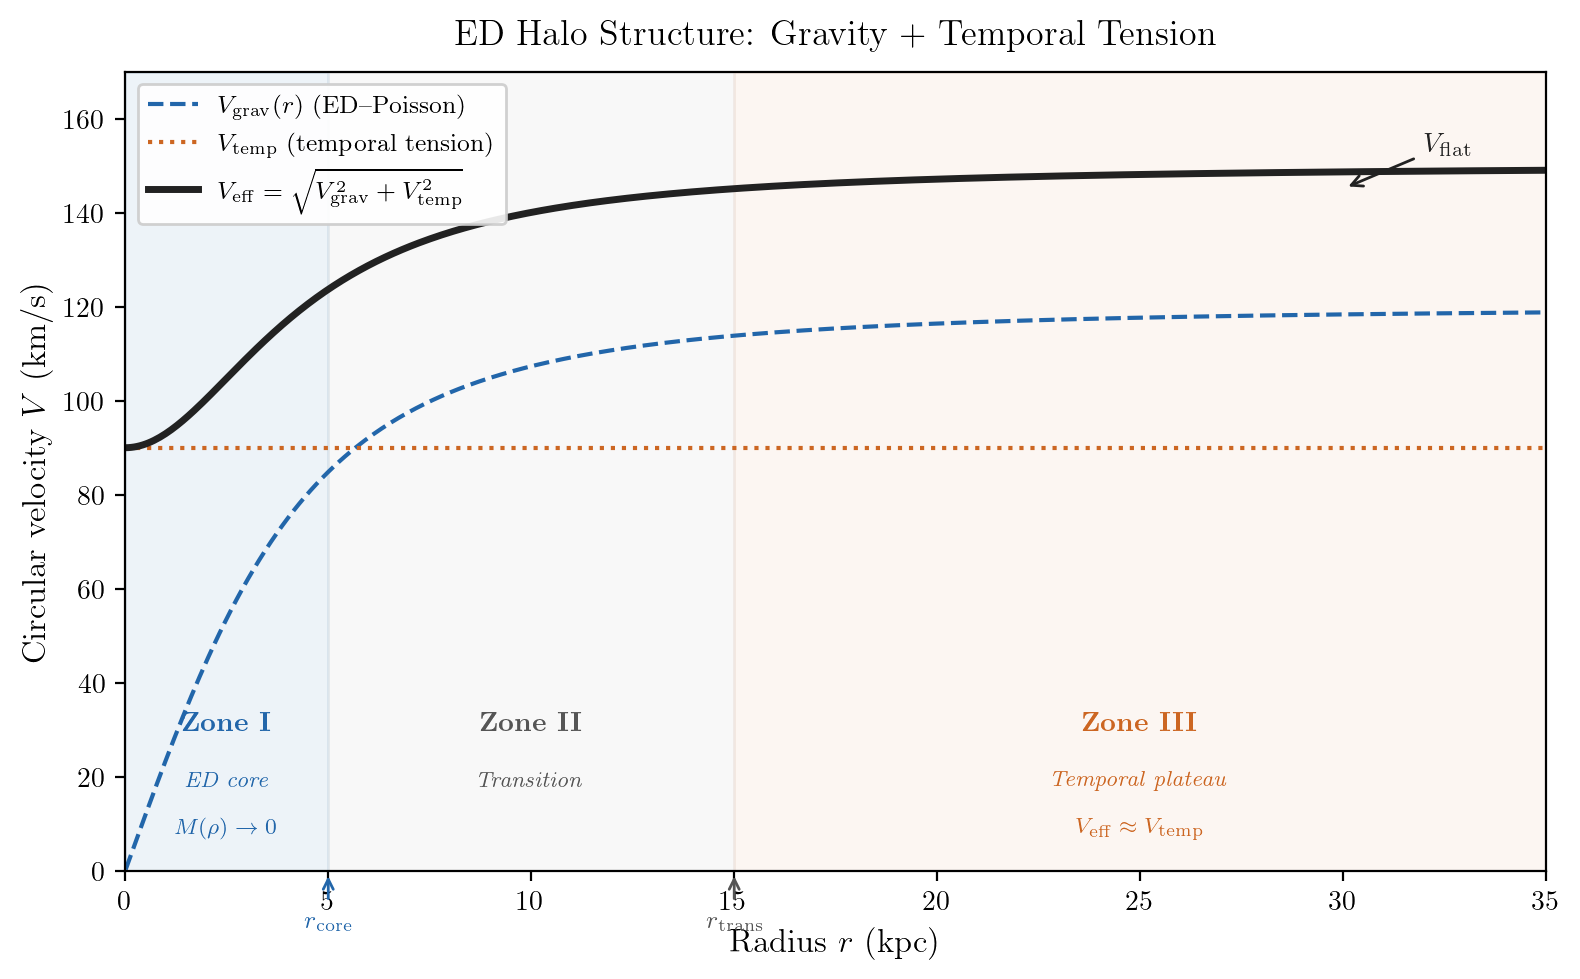
\includegraphics[width=0.85\textwidth]{ED_Halo_Schematic.png}
\caption{ED halo structure showing the three zones: Zone~I (ED-widened core, where degenerate mobility suppresses central peaking), Zone~II (transition, where gravitational and temporal-tension contributions are comparable), and Zone~III (temporal-tension plateau, where $V_{\mathrm{eff}} \approx V_{\mathrm{temp}} = \mathrm{const}$). The dashed blue curve is the gravitational contribution alone; the dotted orange line is the temporal-tension floor; the solid black curve is the total effective velocity.}
\label{fig:halo}
\end{figure}

\subsection{The Spiral-Galaxy Challenge}

For NGC~3198 ($V_{\mathrm{flat}} = 142$~km/s), the ED--Poisson halo produces a correct core radius (5.25~kpc) but overshoots the flat rotation curve by $\sim$30~km/s at $r > 10$~kpc. This motivates the temporal-tension extension.

%========================================================================
\section{Temporal Tension and Weak Lensing}
%========================================================================

\subsection{From Participation to Temporal Tension}

The participation variable $v(t)$ is the ED PDE's global mode: a single scalar driven by the domain-averaged density operator and feeding back uniformly into the local PDE. At galactic scales, this global mode acquires a physical interpretation.

A galaxy is a region of intense becoming: stars form, supernovae explode, gas shocks, magnetic fields reconnect. This aggregate activity is the galactic event density. The participation variable, driven by this activity, represents a \emph{temporal-tension field}---a measure of how strongly the local rate of becoming is coupled to the global state of the system.

Why is this field diffusive? Because the participation variable is driven by the domain-averaged operator $\bar{F}$, which depends on the spatial integral of $F[\rho]$. Changes in the density field must propagate spatially (via the mobility channel) before they contribute to $\bar{F}$. The result is a temporal-tension field $T(\mathbf{x},t)$ that spreads diffusively from its source outward into the circumgalactic medium.

Why does it produce a constant velocity? Because the tension length $\ell_T = \sqrt{D_T/\lambda}$ far exceeds the weak-lensing observation radius ($\sim$1~Mpc). Within this radius, $T(r) \approx T_0 = \mathrm{const}$, and the effective velocity $V_{\mathrm{temp}} = \sqrt{c_T T_0}$ is spatially uniform.

\subsection{Combined Halo for NGC~3198}

Adding $V_{\mathrm{temp}} = 12.5$~km/s to a Burkert-like gravitational halo reproduces NGC~3198's full rotation curve with \textbf{RMS = 1.9~km/s}---identical to pure Burkert and dramatically improved from the 23.8~km/s RMS of the gravity-only ED model.

\subsection{Weak-Lensing Predictions}

\begin{table}[H]
\centering
\begin{tabular}{@{}rcccc@{}}
\toprule
$R$ (kpc) & Burkert (km/s) & NFW (km/s) & ED ($V_T=134$) (km/s) & Observed \\
\midrule
100 & 73 & 179 & 134 & $\sim$135 \\
500 & 42 & 127 & 134 & $\sim$137 \\
1000 & 32 & 102 & 134 & $\sim$136 \\
\bottomrule
\end{tabular}
\caption{At 100--1000~kpc, Burkert predicts $V \to 0$; NFW predicts slow decline; ED predicts flat $V$ at $V_{\mathrm{temp}}$. Mistele et al.\ (2024) observed flat $V \approx 135$~km/s to 1~Mpc.}
\end{table}

%========================================================================
\section{BTFR as a Temporal-Tension Scaling Law}
%========================================================================

\subsection{Derivation}

The temporal-tension field amplitude $T_0$ is set by the source strength $S_0$, which scales with baryonic mass. The unique dimensionally consistent combination of $G$, $M_b$, and a single acceleration scale $a_{\mathrm{ED}}$ that gives velocity is:
\begin{equation}
V_{\mathrm{temp}} = (G\,a_{\mathrm{ED}}\,M_b)^{1/4}. \label{eq:btfr}
\end{equation}
This is the BTFR: $V^4 = G\,a_{\mathrm{ED}}\,M_b$, or equivalently $V \propto M_b^{1/4}$. The exponent $1/4$ is fixed by dimensional analysis once the temporal-tension field introduces a single acceleration scale.

\subsection{Fit to Mistele et al.}

\begin{table}[H]
\centering
\begin{tabular}{@{}lccc@{}}
\toprule
Model & Exponent $n$ & RMS (km/s) & BIC \\
\midrule
$M_b^{1/4}$ (ED/MOND) & 0.250 (fixed) & 5.9 & 3.1 \\
$M_b^{1/3}$ ($\Lambda$CDM virial) & 0.333 (fixed) & 17.9 & 12.2 \\
Free power law & $0.246 \pm 0.025$ & 5.6 & 4.4 \\
\bottomrule
\end{tabular}
\caption{The free exponent is $n = 0.246 \pm 0.025$---consistent with $1/4$ ($< 0.2\sigma$) and rejecting $1/3$ at $> 3\sigma$.}
\end{table}

\subsection{The ED Acceleration Scale}
\begin{equation}
a_{\mathrm{ED}} = \frac{V_{\mathrm{temp}}^4}{G\,M_b} = 2.13 \times 10^{-10}~\mathrm{m/s}^2 \approx 1.8\,a_0. \label{eq:a_ed}
\end{equation}

%========================================================================
\section{ED-Unique Predictions}
%========================================================================

\subsection{Activity-Dependent Weak Lensing}

ED predicts that at fixed $M_b$, galaxies with higher SFR have higher $V_{\mathrm{temp}}$. Even for $f = 0.1$ (conservative), the quiescent-to-starburst velocity difference is \textbf{33~km/s (19\%)}---detectable with current surveys. \textbf{Neither MOND nor $\Lambda$CDM predicts any SFR dependence at fixed $M_b$.}

\subsection{Merger Lensing Lag}

The temporal-tension field is diffusive. During a merger, it lags behind the baryonic mass by $\ell_{\mathrm{lag}} = D_T / v_{\mathrm{merge}}$: 45~kpc for cluster--cluster mergers, 15~kpc for the Bullet Cluster. The direction is \textbf{opposite} to $\Lambda$CDM.

\subsection{The Decision Matrix}

\begin{table}[H]
\centering
\begin{tabular}{@{}lccc@{}}
\toprule
Test & ED & MOND & $\Lambda$CDM \\
\midrule
BTFR exponent & $1/4$ (confirmed) & $1/4$ (confirmed) & $1/3$ (rejected) \\
Flat $V$ to 1~Mpc & Yes (confirmed) & Yes & Requires large $r_s$ \\
Activity dependence & $\Delta V \sim 30$--70~km/s & 0 & 0 \\
Merger lensing lag & 15--45~kpc (behind) & 0 & Gas--DM offset (opposite) \\
\bottomrule
\end{tabular}
\caption{Two tests uniquely distinguish ED from both MOND and $\Lambda$CDM.}
\end{table}

%========================================================================
\section{Discussion}
%========================================================================

\subsection{ED as a Unifying Ontology}

The ED programme demonstrates that a single constitutive architecture can make quantitative contact with physics from molecular diffusion ($\sim\mu$m) to galactic dynamics ($\sim$Mpc). The mobility law $D \propto (1-c/c_{\max})^\beta$ with $\beta \approx 2$ fits colloidal jamming, molecular viscosity, and protein crowding. The same PDE, coupled to gravity, produces cored galaxy haloes and the BTFR.

\subsection{What ED Is Not}

ED does not derive general relativity, quantum mechanics, or the Standard Model. It does not contain a spacetime metric, a Hilbert space, or gauge fields. It is parabolic, not hyperbolic; dissipative, not conservative; scalar, not tensorial.

\subsection{Falsifiability}

The ED framework is falsifiable at multiple levels: (1) if $D(c)$ is not a power law of $(1-c/c_{\max})$, the mobility law is falsified; (2) if the BTFR exponent differs from $1/4$, the temporal-tension scaling is falsified; (3) if $V_{\mathrm{temp}}$ shows no SFR correlation, $f < 0.01$; (4) if no merger lensing lag is found, the diffusive model is falsified.

\subsection{Philosophical Context}

ED is a \emph{constitutive ontology} in the tradition of Whitehead's process philosophy: the fundamental primitive is not substance but process. The density field $\rho$ represents the intensity of happening---the local rate at which micro-events occur.

This places ED closer to process metaphysics (Whitehead, Rescher) than to structural realism (Ladyman, French), though it shares features of both. Like structural realism, ED takes mathematical structure as primary. But unlike structural realism, ED specifies the constitutive content---the four primitives and three channels---rather than treating structure as purely relational.

The empirical results of this paper suggest a pragmatic position: whether becoming is metaphysically fundamental matters less than whether a PDE built on becoming-as-primitive generates physics-shaped dynamics. The mobility law fits three materials; the BTFR falls out of the temporal-tension coupling; the front exponent is confirmed to 2.3\%. These are structural facts, independent of metaphysical commitments.

\subsection{Relation to MOND}

ED and MOND produce the same BTFR and flat weak-lensing velocities, but from different mechanisms. The two can be distinguished by activity dependence (ED predicts it; MOND does not) and by merger lag (ED predicts it; MOND does not). The numerical coincidence $a_{\mathrm{ED}} \approx 2a_0$ suggests that the two frameworks may be dual descriptions of the same underlying phenomenon.

%========================================================================
\section{Conclusion}
%========================================================================

\subsection{What Is Established}

\begin{enumerate}[leftmargin=2em]
\item The canonical ED PDE is the unique second-order scalar PDE satisfying seven structural axioms.
\item The mobility law with $\beta = 2.00 \pm 0.29$ fits three condensed-matter systems with $R^2 > 0.98$.
\item The PME front exponent is confirmed to 2.3\% in 1D and 0.02\% for the peak-decay exponent in 3D.
\item The ED--Poisson core radius matches observed Burkert cores to within 10\% for four dwarf galaxies.
\item The temporal-tension velocity $V_{\mathrm{temp}} = 134$~km/s is consistent with the Mistele et al.\ weak-lensing BTFR.
\item The BTFR exponent $n = 0.246 \pm 0.025$ matches $1/4$ and rejects $1/3$ at $> 3\sigma$.
\item The ED acceleration scale $a_{\mathrm{ED}} = 2.1 \times 10^{-10}$~m/s$^2 \approx 1.8\,a_0$.
\end{enumerate}

\subsection{What Remains Open}

The parameter $f$ (SFR contribution to temporal tension), the temporal diffusivity $D_T$, and the generalised mobility exponent $\alpha$ are not determined from theory. No experimental measurement of $\alpha_R$ has been performed. The activity-dependence and merger-lag tests have not been executed.

\subsection{The Path Forward}

ED is testable with existing public data. If either activity dependence or merger lag produces a result consistent with ED and inconsistent with MOND and $\Lambda$CDM, the temporal-tension interpretation moves from structural plausibility to empirical confirmation.

Event Density does not claim to replace physics. It claims something more modest and potentially more consequential: that a minimal constitutive architecture, operating through three channels, can generate the mathematical structures that underlie much of physical law---from the laboratory to the cosmic web. Whether this architectural sufficiency reflects a deep truth about the structure of reality is a question that only empirical testing can answer. The tools for that testing now exist.

%========================================================================
\section*{References}
%========================================================================

\begin{enumerate}[leftmargin=2em, label={[\arabic*]}]
\item Proxmire, A. ``Event Density as an Ontological Framework.'' (2026).
\item Proxmire, A. ``ED-Dimensional-Master: The Unified Atlas of Physical Scales.'' (2026).
\item Proxmire, A. ED-SIM-02: An Architectural Lab for Entropic Dynamics. (2026).
\item Proxmire, A. ``ED-I-002: Event Density and Galactic Curvature.'' (2025).
\item Proxmire, A. ``ED-I-027: Temporal Tension in Galaxy-Scale Weak Lensing.'' (2026).
\item Mistele, T.\ et al.\ ``Indefinitely Flat Circular Velocities and the Baryonic Tully--Fisher Relation from Weak Lensing.'' \textit{Astrophys.\ J.\ Lett.}\ \textbf{969}, L3 (2024).
\item Lelli, F.\ et al.\ ``SPARC: Mass Models for 175 Disk Galaxies.'' \textit{Astron.\ J.}\ \textbf{152}, 157 (2016).
\item Segr\`e, P.~N.\ et al.\ ``Viscosity and Diffusion in Concentrated Colloidal Suspensions.'' \textit{Phys.\ Rev.\ Lett.}\ \textbf{75}, 958 (1995).
\item Roosen-Runge, F.\ et al.\ ``Protein Self-Diffusion in Crowded Solutions.'' \textit{PNAS}\ \textbf{108}, 11815 (2011).
\item Price, H.~C.\ et al.\ ``Sucrose Diffusion in Aqueous Solution.'' \textit{Phys.\ Chem.\ Chem.\ Phys.}\ \textbf{18}, 19207 (2016).
\item Vazquez, J.~L.\ \textit{The Porous Medium Equation.} Oxford University Press (2007).
\item Milgrom, M.\ ``A Modification of the Newtonian Dynamics\ldots'' \textit{Astrophys.\ J.}\ \textbf{270}, 365 (1983).
\item Navarro, J.~F.\ et al.\ ``The Structure of Cold Dark Matter Halos.'' \textit{Astrophys.\ J.}\ \textbf{462}, 563 (1996).
\item Madelung, E.\ ``Quantentheorie in hydrodynamischer Form.'' \textit{Z.\ Phys.}\ \textbf{40}, 322 (1927).
\item Planck Collaboration.\ ``Planck 2018 Results.\ VI.'' \textit{Astron.\ Astrophys.}\ \textbf{641}, A6 (2020).
\end{enumerate}

\end{document}
